\def\mytitle{DIGITAL COMMUNICATIONS}
\def\myauthor{V.GOKULKUMAR}
\def\contact{velicharla@outlook.com}
\def\mymodule{Future Wireless Communication (FWC)}
\documentclass[10pt, a4paper]{article}
\usepackage[a4paper,outer=1.5cm,inner=1.5cm,top=1.75cm,bottom=1.5cm]{geometry}
\twocolumn
\usepackage{gauss}
\usepackage{graphicx}
\graphicspath{{./images/}}
\usepackage[colorlinks,linkcolor={black},citecolor={blue!80!black},urlcolor={blue!80!black}]{hyperref}
\usepackage[parfill]{parskip}
\usepackage{lmodern}
\usepackage{tikz}
\usepackage{bm}
%\documentclass[tikz, border=2mm]{standalone}
\usepackage{karnaugh-map}
%\documentclass{article}
\usepackage{tabularx}
\usepackage{circuitikz}
\usetikzlibrary{calc}
\usepackage{enumitem}
\usepackage{amsmath}
\usepackage{bm,amsmath}
\usepackage{amssymb}
\renewcommand*\familydefault{\sfdefault}
\usepackage{watermark}
\usepackage{lipsum}
\usepackage{xcolor}
\usepackage{listings}
\usepackage{float}
\usepackage{titlesec}
       \usepackage[latin1]{inputenc}
       \usepackage{color}
       \usepackage{array}
       \usepackage{longtable}
       \usepackage{calc}
       \usepackage{multirow}
       \usepackage{hhline}
       \usepackage{ifthen}
       
\providecommand{\sbrak}[1]{\ensuremath{{}\left[#1\right]}}
\titlespacing{\subsection}{1pt}{\parskip}{3pt}
\titlespacing{\subsubsection}{0pt}{\parskip}{-\parskip}
\titlespacing{\paragraph}{0pt}{\parskip}{\parskip}
\newcommand{\figuremacro}[5]{
    \begin{figure}[#1]
        \centering
        \includegraphics[width=#5\columnwidth]{#2}
        \caption[#3]{\textbf{#3}#4}
        \label{fig:#2}
    \end{figure}
}
\providecommand{\brak}[1]{\ensuremath{\left(#1\right)}}

\lstset{
frame=single, 
breaklines=true,
columns=fullflexible
}




\thiswatermark{\centering \put(181,-119.0){
\includegraphics[scale=0.13]{iith_logo3}} }
\title{\mytitle}
\author{\myauthor\hspace{1em}\\\contact\\FWC22034\hspace{6.5em}IITH\hspace{0.5em}\mymodule\hspace{6em}ASSIGNMENT}
\begin{document}



\newtheorem{theorem}{Theorem}[section]
\newtheorem{problem}{Problem}
\newtheorem{proposition}{Proposition}[section]
\newtheorem{lemma}{Lemma}[section]
\newtheorem{corollary}[theorem]{Corollary}
\newtheorem{example}{Example}[section]
\newtheorem{definition}[problem]{Definition}
%\newtheorem{thm}{Theorem}[section] 
%\newtheorem{defn}[thm]{Definition}
%\newtheorem{algorithm}{Algorithm}[section]
%\newtheorem{cor}{Corollary}
\newcommand{\BEQA}{\begin{eqnarray}}
\newcommand{\EEQA}{\end{eqnarray}}
\newcommand{\define}{\stackrel{\triangle}{=}}
\bibliographystyle{IEEEtran}
%\bibliographystyle{ieeetr}
\providecommand{\mbf}{\mathbf}
\providecommand{\pr}[1]{\ensuremath{\Pr\left(#1\right)}}
\providecommand{\qfunc}[1]{\ensuremath{Q\left(#1\right)}}
\providecommand{\sbrak}[1]{\ensuremath{{}\left[#1\right]}}
\providecommand{\lsbrak}[1]{\ensuremath{{}\left[#1\right.}}
\providecommand{\rsbrak}[1]{\ensuremath{{}\left.#1\right]}}
\providecommand{\brak}[1]{\ensuremath{\left(#1\right)}}
\providecommand{\lbrak}[1]{\ensuremath{\left(#1\right.}}
\providecommand{\rbrak}[1]{\ensuremath{\left.#1\right)}}
\providecommand{\cbrak}[1]{\ensuremath{\left\{#1\right\}}}
\providecommand{\lcbrak}[1]{\ensuremath{\left\{#1\right.}}
\providecommand{\rcbrak}[1]{\ensuremath{\left.#1\right\}}}
%\theoremstyle{remark}
\providecommand{\abs}[1]{\vert#1\vert}
\newtheorem{rem}{Remark}
\newcommand{\sgn}{\mathop{\mathrm{sgn}}}
%\providecommand{\abs}[1]{\left\vert#1\right\vert}
\providecommand{\res}[1]{\Res\displaylimits_{#1}} 
\providecommand{\norm}[1]{\lVert#1\rVert}
%\providecommand{\norm}[1]{\lVert#1\rVert}
\providecommand{\mtx}[1]{\mathbf{#1}}
%\providecommand{\mean}[1]{E\left[ #1 \right]}
\providecommand{\gauss}[2]{\mathcal{N}\ensuremath{\left(#1,#2\right)}}
\providecommand{\fourier}{\overset{\mathcal{F}}{ \rightleftharpoons}}
%\providecommand{\hilbert}{\overset{\mathcal{H}}{ \rightleftharpoons}}
\providecommand{\system}{\overset{\mathcal{H}}{ \longleftrightarrow}}
	%\newcommand{\solution}[2]{\vec{Solution:}{#1}}
\newcommand{\solution}{\noindent \textbf{Solution: }}
\newcommand{\cosec}{\,\text{cosec}\,}
\providecommand{\dec}[2]{\ensuremath{\overset{#1}{\underset{#2}{\gtrless}}}}
\newcommand{\myvec}[1]{\ensuremath{\begin{pmatrix}#1\end{pmatrix}}}
\newcommand{\mydet}[1]{\ensuremath{\begin{vmatrix}#1\end{vmatrix}}}
%\numberwithin{equation}{section}
%\numberwithin{equation}{subsection}
%\numberwithin{problem}{section}
%\numberwithin{definition}{section}
\makeatletter
\@addtoreset{figure}{problem}
\makeatother
\let\StandardTheFigure\thefigure
\let\vec\mathbf
%\renewcommand{\thefigure}{\theproblem.\arabic{figure}}
%\renewcommand{\thefigure}{\theproblem}
%\setlist[enumerate,1]{before=\renewcommand\theequation{\theenumi.\arabic{equation}}
%\counterwithin{equation}{enumi}

	\maketitle
 \section{Sum of Independent Random Variables}
 \begin {enumerate}
 \item 
The experiment of rolling the dice was simulated using Python for 10000 samples.  These were generated using Python libraries for uniform distribution. The frequencies for each outcome were then used to compute the resulting pmf, which  is plotted in Figure \ref{fig:dice}.  The theoretical pmf obtained in  is plotted for comparison.  
%
\begin{figure}[!ht]
\centering
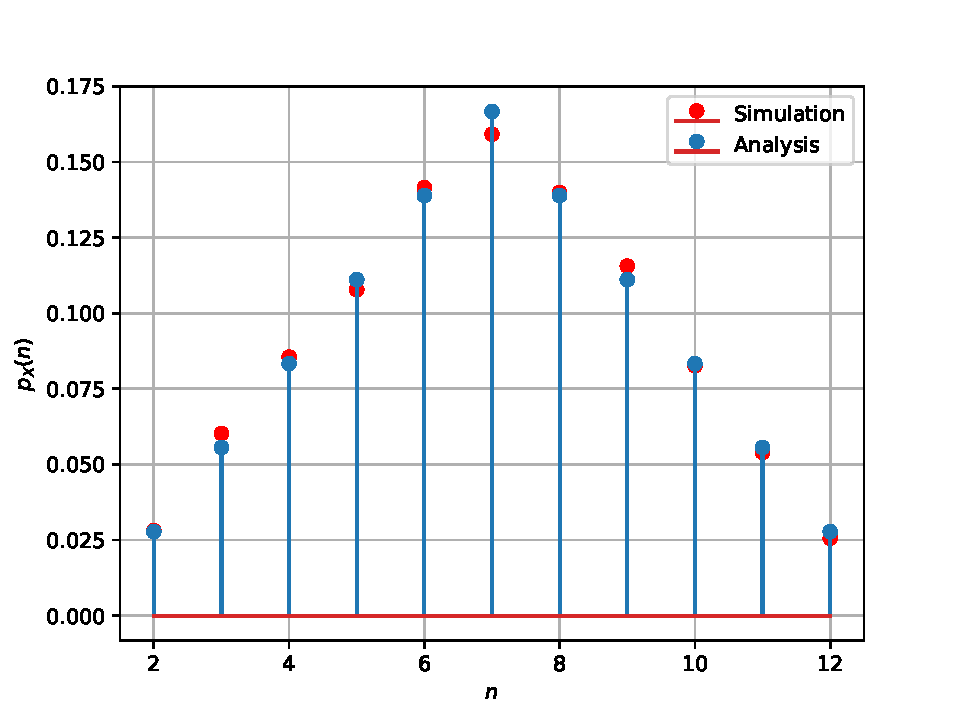
\includegraphics[scale=0.5]{images/4.1.4.pdf}
\caption{Plot of $p_X(n)$.  Simulations are close to the analysis. }
\label{fig:dice}
\end{figure}
\begin{center}
\fbox{\parbox{8.2cm}{\url{https://github.com/velicharlagokulkumar/digital-communications/blob/main/codes/chapter-4/4.1.4/4.1.4.py}}}
\end{center}
\end{enumerate}



	\section{Random numbers}
 \subsection{Uniform Random Numbers}
Let $U$ be a uniform random variable between 0 and 1.
\begin{enumerate}
\item Generate $10^6$ samples of $U$ using a C program and save into a file called uni.dat .

\begin{center}
\fbox{\parbox{8.2cm}{\url{https://github.com/velicharlagokulkumar/digital-communications/blob/main/codes/chapter-5/5.1.1/uni.dat}}}
\end{center}
\item
Load the uni.dat file into python and plot the empirical CDF of $U$ using the samples in uni.dat. The CDF is defined as
\begin{align}
F_{U}(x) = \pr{U \le x}
\end{align}
\\
\solution  The following code plots Fig. \ref{fig:cdf of u}
\begin{center}
\fbox{\parbox{8.2cm}{\url{https://github.com/velicharlagokulkumar/digital-communications/blob/main/codes/chapter-5/5.1.2/cdf_plot.py}}}
\end{center}
\begin{figure}[!ht]
\centering
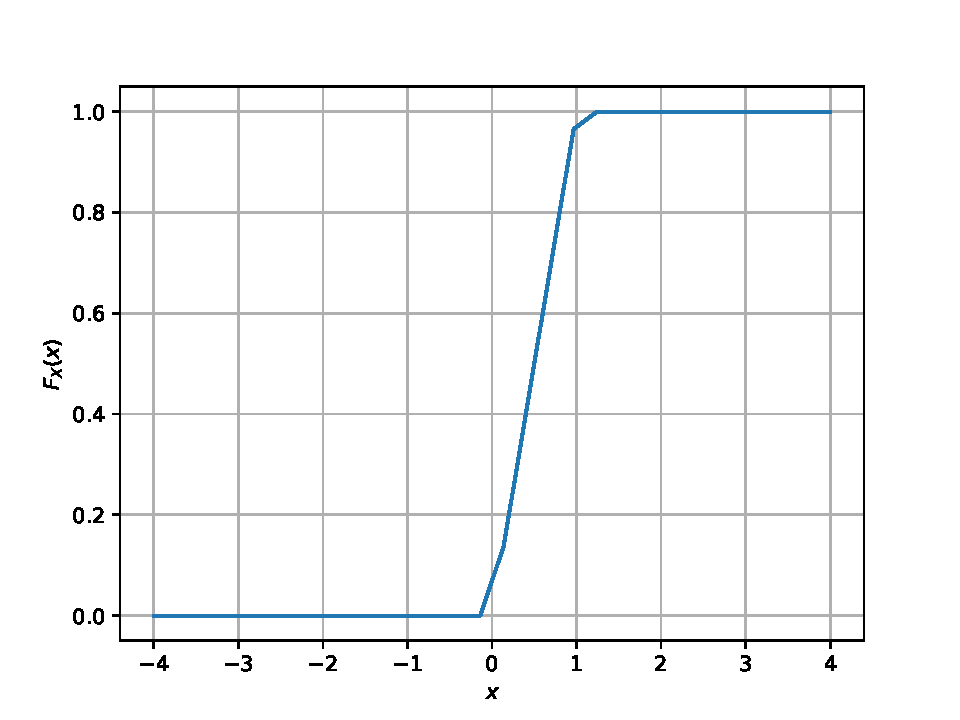
\includegraphics[scale=0.5]{images/uni_cdf.pdf}
\caption{CDF of U}
\label{fig:cdf of u}
\end{figure}
\item
Find a  theoretical expression for $F_{U}(x)$.
\\
Uniform Random variable:
 $$
\begin{aligned}
& \left.\begin{array}{ll}
f_U(x)=\frac{1}{b-a} & a \leq x \leq b \\
\ \ \ \ \ \ \ \ \ =0 & \text { elsewhere }
\end{array}\right\} \begin{array}{l}
\text { where a and } \\
b \text { are real } \\
\text { constants } \\
-\alpha<a<\alpha \\
\& b>a
\end{array} \\
& F_U(x)=\int_{-\infty}^x f_x(x) d x \\
& =\int_{-\infty}^x \frac{1}{b-a} \cdot d x \\
& =\left.\frac{1}{b-a} \cdot x\right|_a ^x \\
& =\frac{x-a}{b-a} \\
\end{aligned}
$$

$$
F_U(x)=\left\{\begin{array}{lr}
0 & x<a \\
(x-a) /(b-a) & a \leq x<b \\
1 & b \leq x
\end{array}\right.
$$

\item
The mean of $U$ is defined as
%
\begin{equation}
E\sbrak{U} = \frac{1}{N}\sum_{i=1}^{N}U_i
\end{equation}
%
and its variance as
%
\begin{equation}
\text{var}\sbrak{U} = E\sbrak{U- E\sbrak{U}}^2 
\end{equation}
Write a C program to  find the mean and variance of $U$. 


\begin{lstlisting}
#include <stdio.h>
#include <stdlib.h>
#include <math.h>
#include "coeffs.h"

int  main(void) //main function begins
{
 
//Uniform random numbers
uniform("uni.dat", 1000000);

//Mean of uniform
printf("%lf\n",mean("uni.dat"));
//Variance of uniform
printf("%lf",variance("uni.dat"));
return 0;
}
\end{lstlisting}
\begin{lstlisting}
double mean(char *str)
{
int i=0,c;
FILE *fp;
double x, temp=0.0;

fp = fopen(str,"r");
//get numbers from file
while(fscanf(fp,"%lf",&x)!=EOF)
{
//Count numbers in file
i=i+1;
//Add all numbers in file
temp = temp+x;
}
fclose(fp);
temp = temp/(i-1);
return temp;

}
\end{lstlisting}
\begin{lstlisting}
double variance(char *str)
{
int i=0,j=0,c;
FILE *fp;
double x, temp=0.0,value,sumsqr=0,variance=0.0;

fp = fopen(str,"r");
//get numbers from file
while(fscanf(fp,"%lf",&x)!=EOF)
{
//Count numbers in file
i=i+1;
//Add all numbers in file
temp = temp+x;
}
fclose(fp);
temp = temp/(i-1);
fp = fopen(str,"r");
while(fscanf(fp,"%lf",&x)!=EOF)
{
  j=j+1;
  value=x-temp;
     sumsqr=sumsqr+value*value;
}
fclose(fp);
variance = sumsqr/(j-1);
return variance;
}
\end{lstlisting}
Result:
\begin{lstlisting}
  mean=0.500137 
  variance=0.83251
\end{lstlisting}
\begin{center}
\fbox{\parbox{8.2cm}{\url{https://github.com/velicharlagokulkumar/digital-communications/blob/main/codes/chapter-5/5.1.4/uniform.c}}}
\end{center}

\item Verify your result theoretically given that
%
\begin{equation}
E\sbrak{U^k} = \int_{-\infty}^{\infty}x^kdF_{U}(x)
\end{equation}
\begin{align}
Mean:
 \mathrm{E}[U]=\int_a^b x \cdot \frac{1}{b-a} d x=\frac{b^2-a^2}{2} \cdot \frac{1}{b-a} \\ =\frac{(b-a)(b+a)}{2} \cdot \frac{1}{b-a} \\=\frac{b+a}{2} 
 \\ Here \  a=0,b=1
 \\ \mu= \mathrm{E}[X]= \frac{1}{2} = 0.5
\\
 \mathrm{E}[U^2]=\int_a^b x^2 \cdot \frac{1}{b-a} d x=\frac{b^3-a^3}{3} \cdot \frac{1}{b-a} \\ =\frac{a^2+ab+b^2}{3}\\
 Variance:
 \sigma^2=E\left(U^2\right)-[E(U)]^2
 =\frac{(a-b)^2}{12}\\
  \sigma^2=0.834
\end{align}
\end{enumerate}

 \subsection{Central Limit Theorem}
 
\begin{enumerate}

%
\item
Generate $10^6$ samples of the random variable
%
\begin{equation}
X = \sum_{i=1}^{12}U_i -6
\end{equation}
%
using a C program, where $U_i, i = 1,2,\dots, 12$ are  a set of independent uniform random variables between 0 and 1
and save in a file called gau.dat

\begin{center}
\fbox{\parbox{8.2cm}{\url{https://github.com/velicharlagokulkumar/digital-communications/blob/main/codes/chapter-5/5.2.1/gau.dat}}}
\end{center}

\item
Load gau.dat in python and plot the empirical CDF of $X$ using the samples in gau.dat. What properties does a CDF have?
\\
\solution The CDF of $X$ is plotted in Fig. \ref{fig:gauss_cdf}
\begin{center}
\fbox{\parbox{8.2cm}{\url{https://github.com/velicharlagokulkumar/digital-communications/blob/main/codes/chapter-5/5.2.2/cdf_plot.py}}}
\end{center}

\begin{figure}
\centering
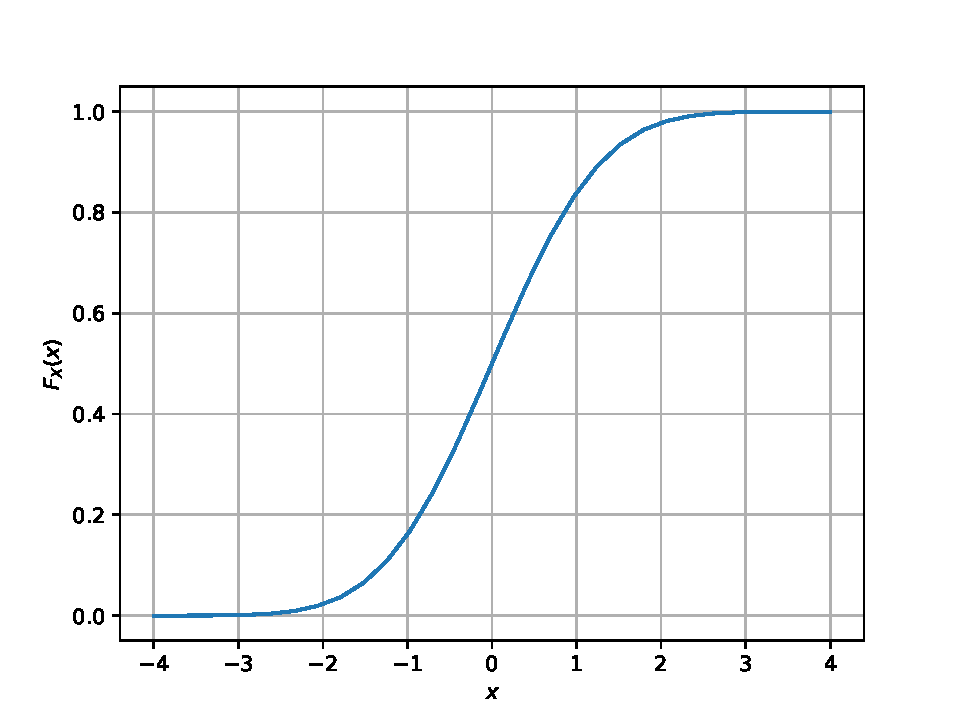
\includegraphics[scale=0.5]{images/gau_cdf.pdf}
\caption{CDF of X}
\label{fig:gauss_cdf}
\end{figure}
\item
Load gau.dat in python and plot the empirical PDF of $X$ using the samples in gau.dat. The PDF of $X$ is defined as
\begin{align}
p_{X}(x) = \frac{d}{dx}F_{X}(x)
\end{align}
What properties does the PDF have?
\\
\solution The PDF of $X$ is plotted in Fig. \ref{fig:gauss_pdf} using the code below
\begin{center}
\fbox{\parbox{8.2cm}{\url{https://github.com/velicharlagokulkumar/digital-communications/blob/main/codes/chapter-5/5.2.3/pdf_plot.py}}}
\end{center}
\begin{figure}
\centering
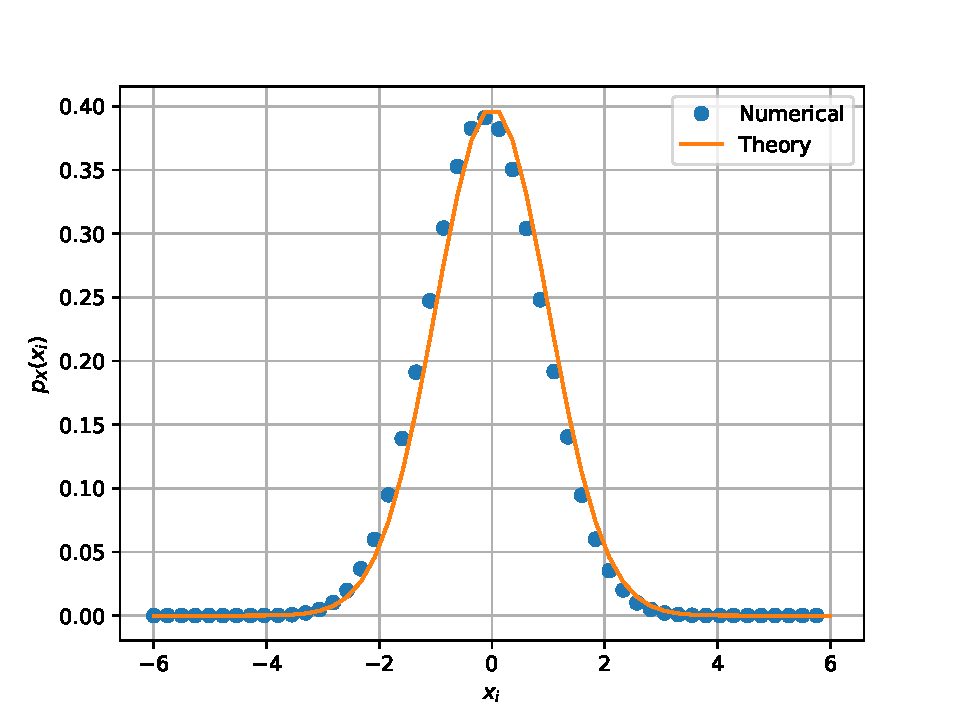
\includegraphics[scale=0.5]{images/gau_pdf.pdf}
\caption{The PDF of $X$}
\label{fig:gauss_pdf}
\end{figure}


 \item Find the mean and variance of $X$ by writing a C program.
\begin{lstlisting}
#include <stdio.h>
#include <stdlib.h>
#include <math.h>
#include "coeffs.h"

int  main(void) //main function begins
{
 
//gaussian random numbers
gaussian("gau.dat", 1000000);

//Mean ,variance of gaussian
printf("%lf\n",mean("gau.dat"));
printf("%lf",variance("gau.dat"));
return 0;
}
\end{lstlisting}
\begin{lstlisting}
double mean(char *str)
{
int i=0,c;
FILE *fp;
double x, temp=0.0;

fp = fopen(str,"r");
//get numbers from file
while(fscanf(fp,"%lf",&x)!=EOF)
{
//Count numbers in file
i=i+1;
//Add all numbers in file
temp = temp+x;
}
fclose(fp);
temp = temp/(i-1);
return temp;

}
\end{lstlisting}
\begin{lstlisting}
double variance(char *str)
{
int i=0,j=0,c;
FILE *fp;
double x, temp=0.0,value,sumsqr=0,variance=0.0;

fp = fopen(str,"r");
//get numbers from file
while(fscanf(fp,"%lf",&x)!=EOF)
{
//Count numbers in file
i=i+1;
//Add all numbers in file
temp = temp+x;
}
fclose(fp);
temp = temp/(i-1);
fp = fopen(str,"r");
while(fscanf(fp,"%lf",&x)!=EOF)
{
  j=j+1;
  value=x-temp;
     sumsqr=sumsqr+value*value;
}
fclose(fp);
variance = sumsqr/(j-1);
return variance;
}


\end{lstlisting}

\begin{lstlisting}
  mean= 0.000283
  variance=0.999702
\end{lstlisting}

\begin{center}
\fbox{\parbox{8.2cm}{\url{https://github.com/velicharlagokulkumar/digital-communications/blob/main/codes/chapter-5/5.2.4/gauss.c}}}
\end{center}

\item Given that 
\begin{align}
p_{X}(x) = \frac{1}{\sqrt{2\pi}}\exp\brak{-\frac{x^2}{2}}, -\infty < x < \infty,
\end{align}
repeat the above exercise theoretically.
$$
\begin{aligned}
& E(X)=\frac{1}{\sqrt{2 \pi}} \int_{-\infty}^{\infty} x e^{-\frac{x^2}{2}} d x \\
& =0 \quad \text { ( odd function) } \\
& E\left(X^2\right)=\frac{1}{\sqrt{2 \pi}} \int_{-\infty}^{\infty} x^2 e^{-\frac{x^2}{2}} d x \quad \text { (evenfunction) } \\
& =\frac{2}{\sqrt{2 \pi}} \int_0^{\infty} x^2 e^{-\frac{x^2}{2}} d x \\
& =\frac{2}{\sqrt{2 \pi}} \int_0^{\infty} \sqrt{2 u} e^{-u} d u \quad\left(\text { Let } \frac{x^2}{2}=u\right) \\
& =\frac{2}{\sqrt{\pi}} \int_0^{\infty} e^{-u} u^{\frac{3}{2}-1} d u \\
& =\frac{2}{\sqrt{\pi}} \Gamma\left(\frac{3}{2}\right) \\
& =\frac{1}{\sqrt{\pi}} \Gamma\left(\frac{1}{2}\right) \\
& =1 \\
&
\end{aligned}
$$
where we have used the fact that
$$
\because \Gamma(n)=(n-1) \Gamma(n-1) ; \Gamma\left(\frac{1}{2}\right)=\sqrt{\pi}
$$
Thus, the variance is
$$
\sigma^2=E(X)^2-E^2(X)=1
$$
\end{enumerate}




\subsection{From Uniform to Other}
\begin{enumerate}
\item Generate samples of 
%
\begin{equation}
V = -2\ln\brak{1-U}
\label{eq:probman_V_cdf_sim}
\end{equation}
%
and plot its CDF.
\begin{figure}[!ht]
\centering
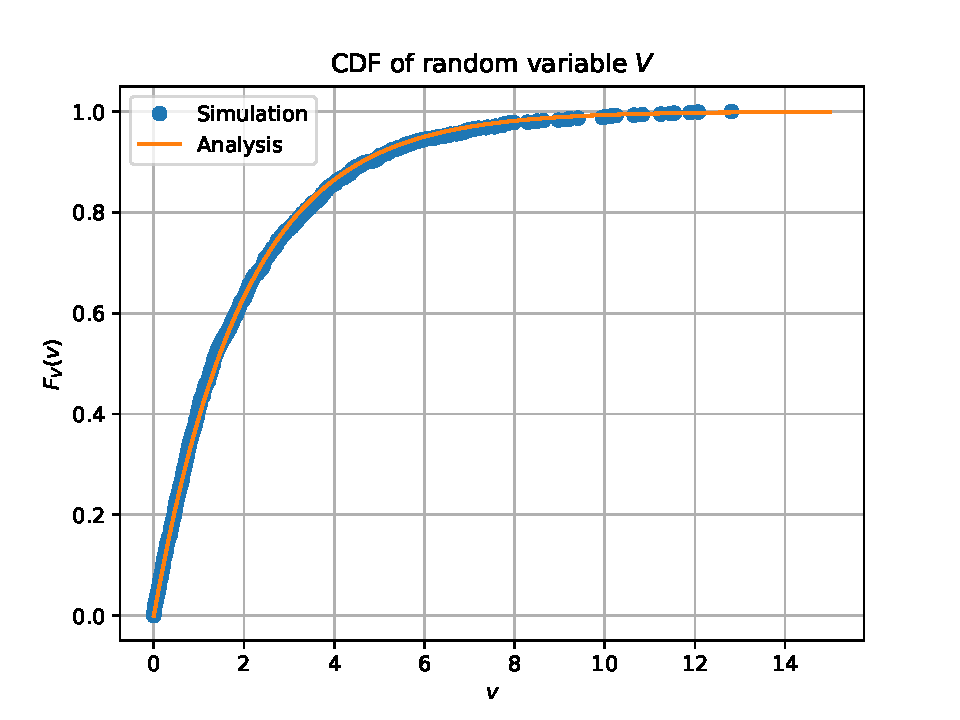
\includegraphics[scale=0.5]{images/5.3.pdf}
\caption{CDF of V}
\end{figure}

\begin{center}
\fbox{\parbox{8.2cm}{\url{https://github.com/velicharlagokulkumar/digital-communications/blob/main/codes/chapter-5/5.3/5.3.py}}}
\end{center}

\item Find a theoretical expression for $F_V(x)$.
The CDF of $V$ is defined as 
\begin{align}
    F_V(v) &= \pr{V \le v}\\
           &= \pr{-2 \ln(1-U)\le v} \\
           &= \pr{\ln(1-U) \ge -\frac{v}{2}}\\
           &= \pr{1-U \ge \exp\brak{-\frac{v}{2}}}\\
           &= \pr{U \le 1- \exp\brak{-\frac{v}{2}}}\\
           &= F_U\brak{1- \exp\brak{-\frac{v}{2}}}
%           &=  (1-(exp(-v/2))
\label{eq:probman_cdf_V_temp}
\end{align}
\begin{align}
F_U(x) = 
\begin{cases}
0 &  x < 0 \\
x & 0 \le x \le 1 \\
1 & x > 1
\end{cases}
\end{align}
%
Substituting the above in \eqref{eq:probman_cdf_V_temp},
%
\begin{multline}
F_U\brak{1- \exp\brak{-\frac{v}{2}}} =
\\
\begin{cases}
0 &  1- \exp\brak{-\frac{v}{2}} < 0 \\
1- \exp\brak{-\frac{v}{2}} & 0 \le 1- \exp\brak{-\frac{v}{2}} \le 1 \\
1 & 1- \exp\brak{-\frac{v}{2}} > 1
\end{cases}
\end{multline}
%
After some algebra, the above conditions yield
\begin{align}
F_V(v) = 
\begin{cases}
0 & v < 0 \\
1- exp\brak{-\frac{v}{2}} & v \ge 0
\end{cases}
\label{eq:probman_V_cdf_anal}
\end{align}
%
which is the CDF of the exponential distribution with parameter $\frac{1}{2}$. 
\end{enumerate}


\subsection{Triangular Distribution}
\begin{enumerate}[label=\thesection.\arabic*
,ref=\thesection.\theenumi]
%
\item Generate 
	\begin{align}
		Z = U_1+U_2
	\end{align}


 \begin{center}
\fbox{\parbox{8cm}{\url{https://github.com/velicharlagokulkumar/digital-communications/blob/main/codes/chapter-5/5.4/uniform_two.c}}}
\end{center}


\item Find the CDF of $Z$.
 \begin{center}
\fbox{\parbox{8cm}{\url{https://github.com/velicharlagokulkumar/digital-communications/blob/main/codes/chapter-5/5.4/5.4_cdf.py}}}
\end{center}
\begin{figure}[!ht]
\centering
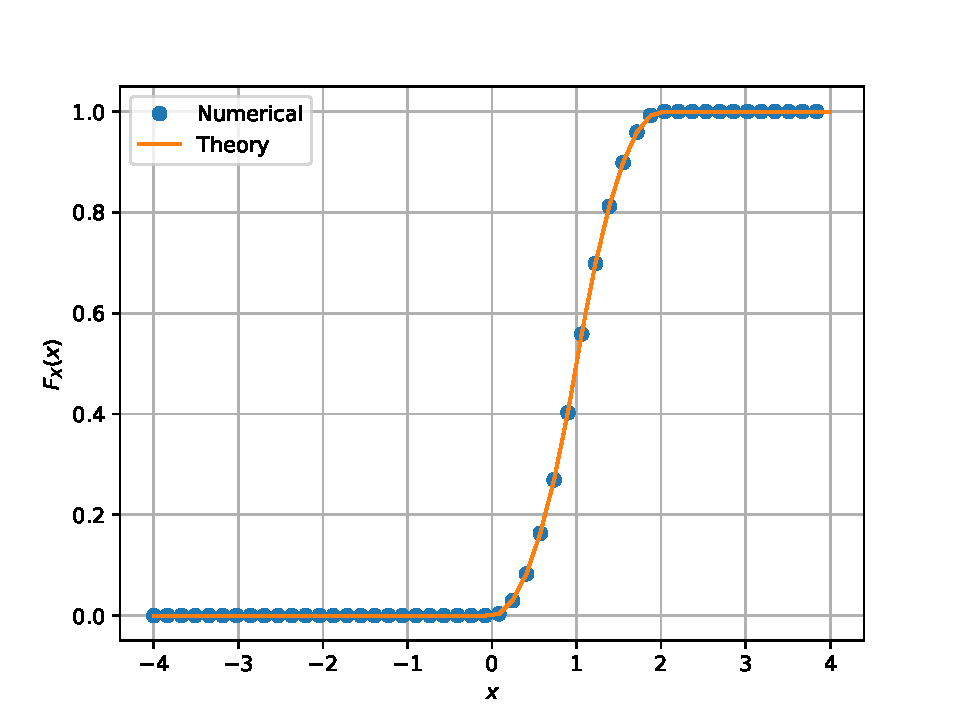
\includegraphics[scale=0.5]{images/5.4_cdf.pdf}
\caption{CDF of Z}
\label{fig_6}
\end{figure}

\item Find the PDF of $Z$.
 \begin{figure}[!ht]
\centering
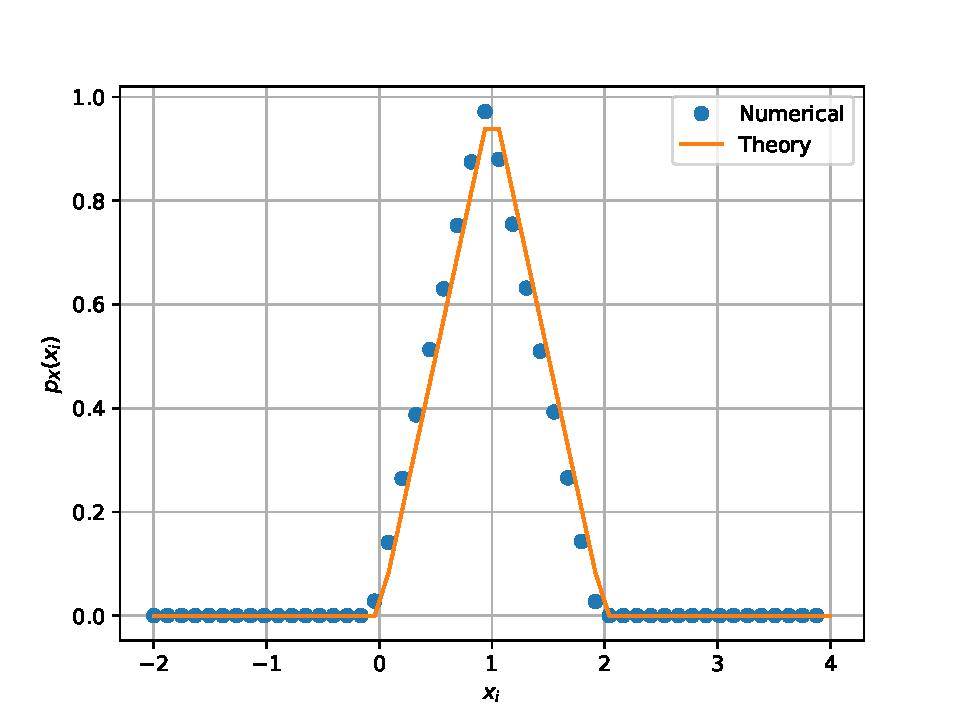
\includegraphics[scale=0.5]{images/5.4_pdf.pdf}
\label{fig_7}
\caption{PDF of Z}
\end{figure}

 
 \begin{center}
\fbox{\parbox{8.2cm}{\url{https://github.com/velicharlagokulkumar/digital-communications/blob/main/codes/chapter-5/5.4/5.4_pdf.py}}}
\end{center}
\item Find the theoretical expressions for the PDF and CDF of $Z$.
\begin{align}
f(z) = 
\begin{cases}
z & 0 < z < 1  \\
2-z & 1 \le z < 2 \\
0 & otherwise
\end{cases}
\end{align}

\begin{align}
F_Z(z) = 
\begin{cases}
\frac{z^2}{2} & 0 < z < 1  \\
2z-z^2-1 & 1 \le z < 2 \\
1 & z>0
\end{cases}
\end{align}


\item Verify your results through a plot. \\
\solution
 From Figure:6,Figure:7
\end{enumerate}







\section{transfromations of R.V}
\subsection{Gaussian to Other}
\begin{enumerate}
\item
Let $X_1 \sim  (0,1) $ and $X_2 \sim (0,1)$. Plot the CDF and PDF of
%
\begin{equation}
V = X_1^2 + X_2^2 
\end{equation}

\begin{center}
\fbox{\parbox{8.2cm}{\url{https://github.com/velicharlagokulkumar/digital-communications/blob/main/codes/chapter-8/8.1.1/8.1.1_CDF.py}}}
\end{center}
\begin{center}
\fbox{\parbox{8.2cm}{\url{https://github.com/velicharlagokulkumar/digital-communications/blob/main/codes/chapter-8/8.1.1/8.1.1_PDF.py}}}
\end{center}


\begin{figure}[!ht]
\centering
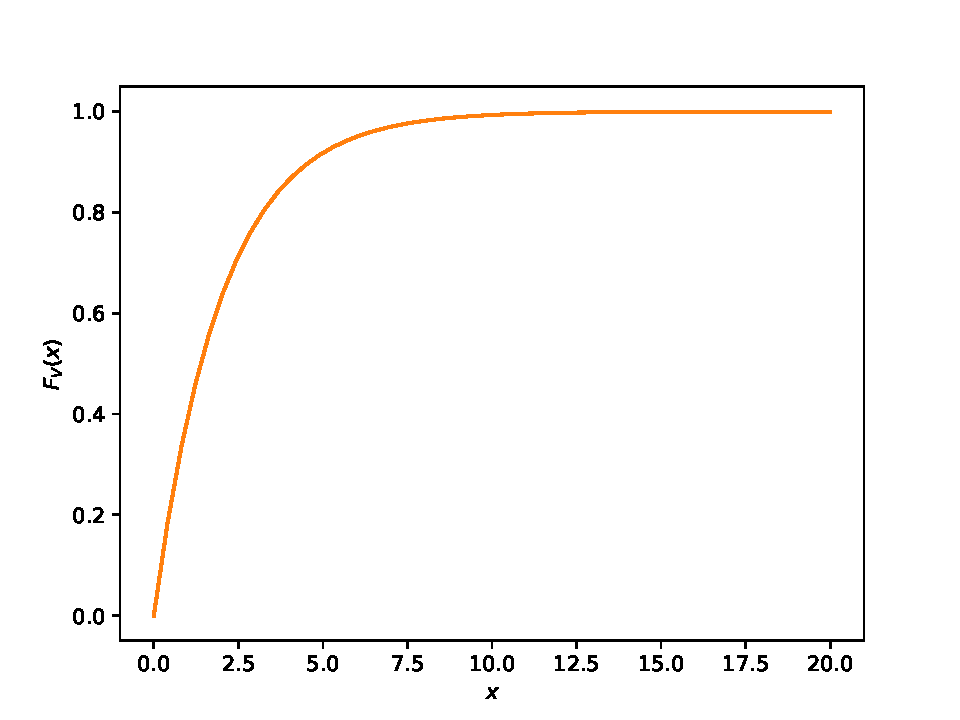
\includegraphics[scale=0.5]{images/7.1.1_CDF.pdf}
\caption{CDF of $V$}
\end{figure}

\begin{figure}[!ht]
\centering
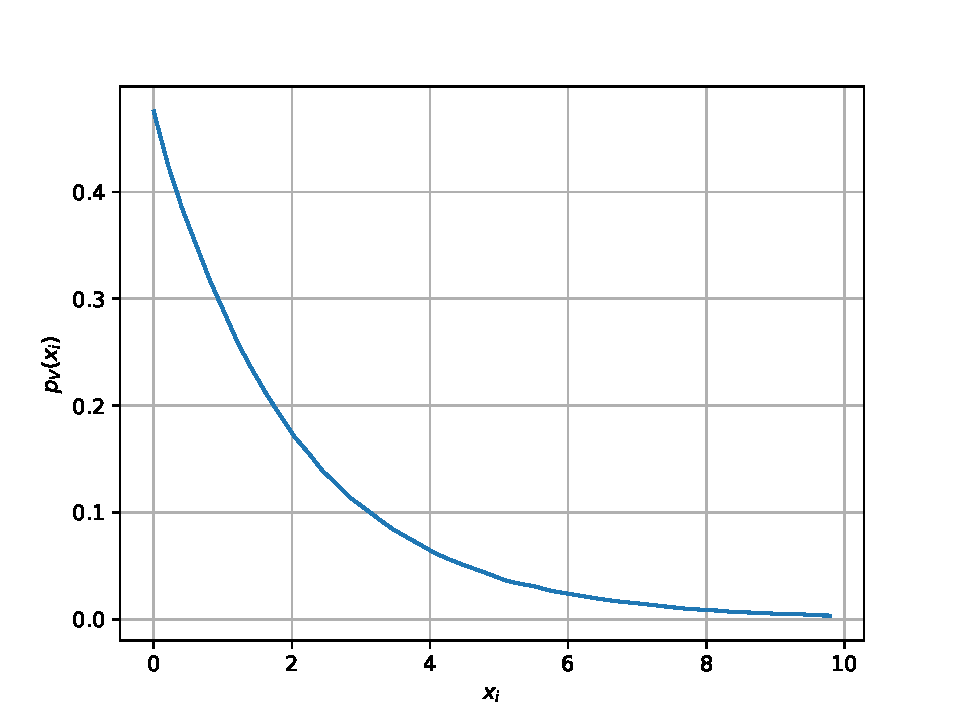
\includegraphics[scale=0.5]{images/7.1.1_PDF.pdf}
\caption{PDF of $V$}
\end{figure}




\item
If
%
\begin{equation}
F_{V}(x) = 
\begin{cases}
1 - e^{-\alpha x} & x \geq 0 \\
0 & x < 0,
\end{cases}
\label{eq:probman_F_V_alpha}
\end{equation}
%
find $\alpha$.
\\
\solution
For the value $\alpha=0.5$, the theory matches the simulation.  

The following code generates the CDF of $V$ in Fig. \ref{cdf_v}

\begin{figure}[!ht]
\centering
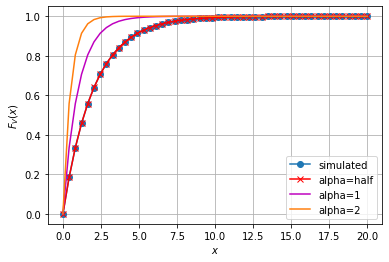
\includegraphics[scale=0.5]{images/7.1.2.png}
\caption{CDF of $V$}
\label{cdf_v}
\end{figure}

\begin{center}
\fbox{\parbox{8.2cm}{\url{https://github.com/velicharlagokulkumar/digital-communications/blob/main/codes/chapter-8/8.1.2/8.1.2.py}}}
\end{center}





%
%
\item
\label{ch3_raleigh_sim}
Plot the CDF and PDf of
%
\begin{equation}
A = \sqrt{V}
\end{equation}

$$
\begin{aligned}
F_A(a) & =\Pr{\left(A<a\right) } \\
& =\Pr{\left(\sqrt{V}<a\right)} \\
& =\Pr{\left(V<a^2\right)} \\
& =F_V\left(a^2\right) \\
& =1-\exp \left(-\frac{a^2}{2}\right)\\
f(a)&=a \exp \left(-\frac{a^2}{2}\right)
\end{aligned}
$$
 The CDF and PDF of A are plotted in Figs. \ref{fig:probman_trans_cdf_A} and \ref{fig:probman_trans_PDf_A}
using the codes below.

\begin{figure}[!ht]
\centering
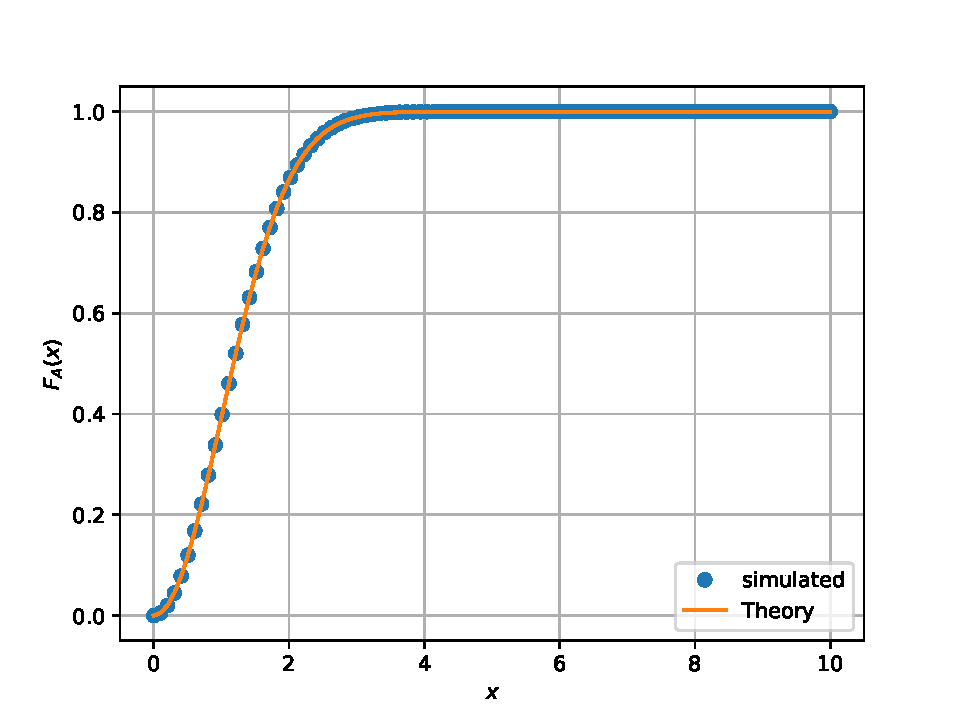
\includegraphics[scale=0.5]{images/7.1.3_CDF.pdf}
\caption{CDF of A}
\label{fig:probman_trans_cdf_A}
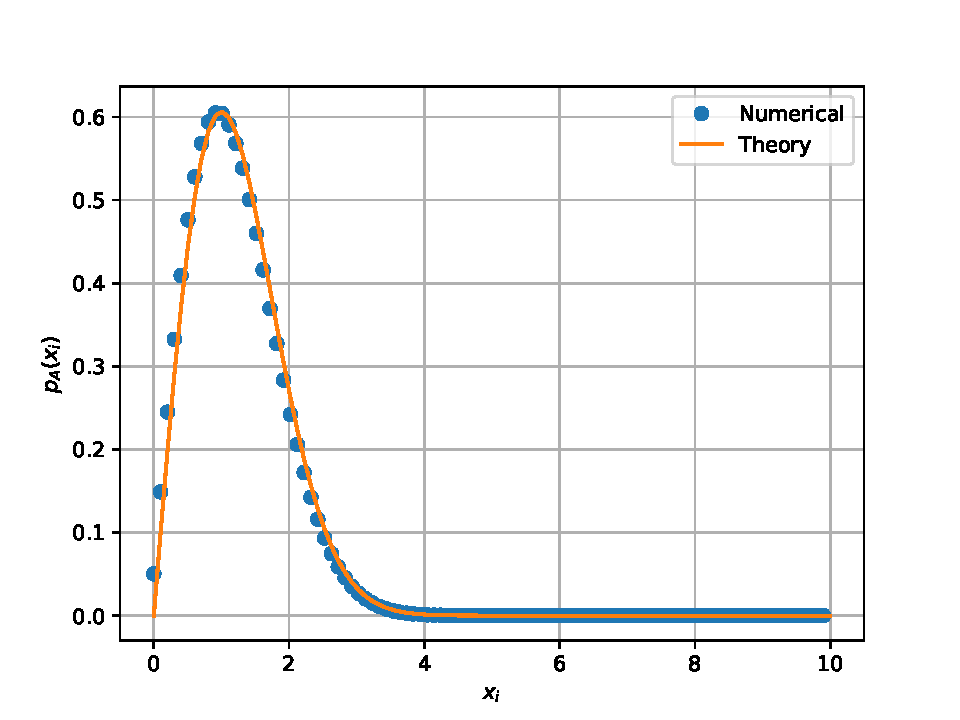
\includegraphics[scale=0.5]{images/7.1.3_PDF.pdf}
\caption{PDF of A}
\label{fig:probman_trans_PDf_A}
\end{figure}

\end{enumerate}
\begin{center}
\fbox{\parbox{8.2cm}{\url{https://github.com/velicharlagokulkumar/digital-communications/blob/main/codes/chapter-8/8.1.3/8.1.3_CDF.py}}}
\end{center}
\begin{center}
\fbox{\parbox{8.2cm}{\url{https://github.com/velicharlagokulkumar/digital-communications/blob/main/codes/chapter-8/8.1.3/8.1.3_PDF.py}}}
\end{center}

\subsection{Conditional Probability}
\begin{enumerate}
\item
\label{ch4_sim}
Plot 
\begin{equation}
P_e = \pr{\hat{X} = -1|X=1}
\end{equation}
%
for 
\begin{equation}
Y = AX+N,
\end{equation}
where $A$ is Raleigh with $E\sbrak{A^2} = \gamma, N \sim \mathcal{N}(0,1) \in \brak{-1,1}$ for $0 \le \gamma \le 10$ dB.
\\


%
\item
Assuming that $N$ is a constant, find an expression for $P_e$.  Call this $P_e(N)$.
\\
\solution
The estimated value $\hat{X}$ is given by
\begin{align}
\hat{X} = 
\begin{cases}
+1 & Y>0\\
-1 & Y<0
\end{cases}
\end{align}
For $X = 1$, 
\begin{align}
Y &= A + N\\
P_e &= \pr{\hat{X} = -1|X=10} \\
&=\pr{Y<0 |X=1}\\
&= \pr{A<-N)}\\
&= F_A(-N)\\
&= \int_{-\infty}^{-N} f_A(x)dx
\end{align}
By definition
\begin{align}
f_A(x) = 
\begin{cases}
\frac{x}{\sigma^2}\exp\brak{{-\frac{x^2}{2\sigma^2}}} & x\geq0\\
0 & otherwise
\end{cases}
\end{align}
If $N>0, f_A(x) = 0$. Then,
\begin{align}
 P_e=0  
\end{align}
If $N<0$. Then,
\begin{align}
 P_e(N) &=\int_{-\infty}^{-N} f_A(x)dx\\
 &=\int_{-\infty}^{0} 0dx+\int_{0}^{-N} f_A(x)dx\\
 &=\int_{0}^{-N} \frac{x}{\sigma^2}\exp\brak{{-\frac{x^2}{2\sigma^2}}}dx\\
 &=1-\exp{\brak{-\frac{N^2}{2\sigma^2}}}
\end{align}
Therefore,
\begin{align}\label{pe(N)}
P_e(N) = 
\begin{cases}
1-\exp\brak{{-\frac{N^2}{2\sigma^2}}} & N<0\\
0 & otherwise
\end{cases}
\end{align}
%

%
\item
%
\label{ch4_anal}
For a function $g$,
\begin{equation}
E\sbrak{g(X)} = \int_{-\infty}^{\infty}g(x)p_{X}(x)\, dx
\end{equation}
%
Find $P_e = E\sbrak{P_e(N)}$.
\\
\solution
Since $N \sim \mathcal{N}(0,1)$ ,
\begin{align}
  p_N(x)= \frac{1}{\sqrt{2\pi}}\exp \brak{-\frac{x^2}{2} }\\
\end{align}
And from \eqref{pe(N)} 
\begin{align}
    P_e(x)=
    \begin{cases}
1-\exp\brak{{-\frac{x^2}{2\sigma^2}}} & x<0\\
0 & otherwise
\end{cases}
\end{align}

\begin{align}
 P_e=E\sbrak{P_e(N)} = \int_{-\infty}^{\infty}P_e(x)p_{N}(x)\, dx  
\end{align}
If $x<0, P_e(x)=0$ and using the fact that for an even function
\begin{align}
\int_{-\infty}^{\infty}f(x)=2\int_{-\infty}^{0}f(x)   
\end{align}
we get
\begin{align}
  P_e&= \frac{1}{\sqrt{2\pi}}\int_{-\infty}^{0}\exp \brak{ -\frac{x^2}{2}} \brak{1-\exp \brak{ -\frac{x^2}{2\sigma^2}} } dx\\
&= \frac{1}{2\sqrt{2\pi}} \int_{-\infty}^{\infty} \exp \brak{ -\frac{x^2}{2} }dx \nonumber \\
&- \frac{1}{2\sqrt{2\pi}} \int_{-\infty}^{\infty} \exp \brak{-\frac{(1+ \sigma^2)x^2}{2 \sigma^2}}  dx\\
&= \frac{\sqrt{2\pi} - \sqrt{\frac{\pi(2\sigma^2)}{1+\sigma^2}}}{2\sqrt{2\pi}}\\
&= \frac{1}{2} - \frac{1}{2}\sqrt{\frac{\sigma^2}{1+\sigma^2}}
\end{align}
For a Rayleigh Distribution with scale $= \sigma$,
\begin{align}
E\sbrak{A^2} = 2\sigma^2\\
\gamma = 2\sigma^2\\
\therefore P_e = \frac{1}{2} - \frac{1}{2}\sqrt{\frac{\gamma}{2+\gamma}}
\end{align}
%
%
\item
Plot $P_e$ in problems \ref{ch4_sim} and \ref{ch4_anal} on the same graph w.r.t $\gamma$.  Comment.
\\
\begin{center}
\fbox{\parbox{8.2cm}{\url{https://github.com/velicharlagokulkumar/digital-communications/blob/main/codes/chapter-8/8.2/8.2.py}}}
\end{center}
\begin{figure}[!ht]
\centering
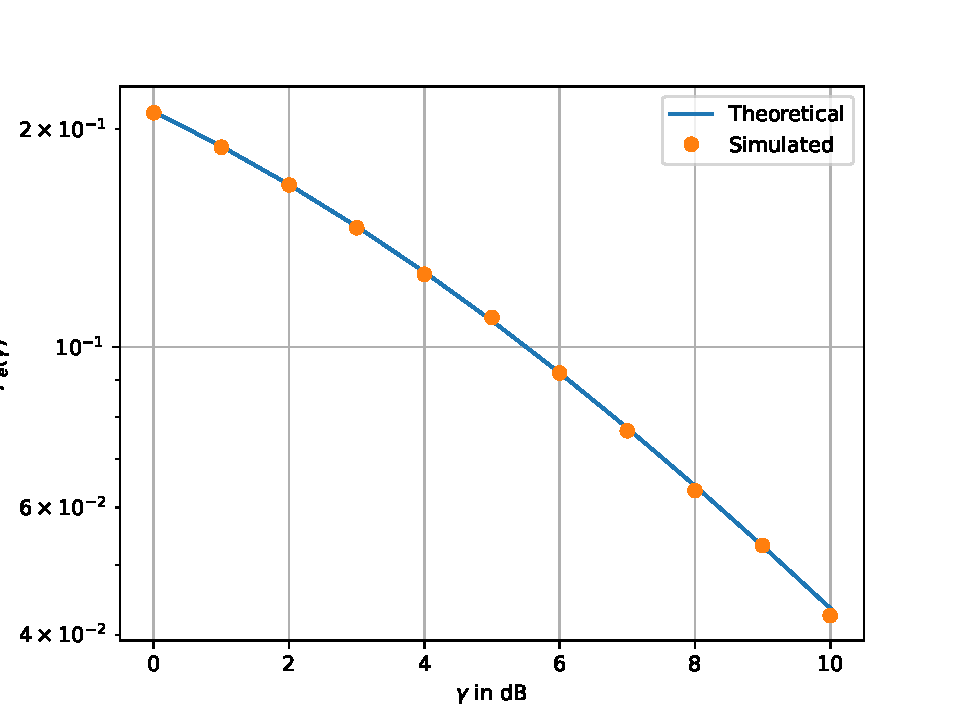
\includegraphics[scale=0.5]{images/7.2.pdf}
\end{figure}
\end{enumerate}





\section{Maximum Likelihood Detection:BPSK}
\subsection{Maximum Likelihood}
\begin{enumerate}
\item Generate equiprobable $X \in \cbrak{1,-1}$,$Y = AX+N$ \\ Plot $Y$ using a scatter plot.\\
		where $A = 5$ dB,  and $N \sim \gauss{0}{1}$.\\
  \solution  
\begin{center}
\fbox{\parbox{8.2cm}{\url{https://github.com/velicharlagokulkumar/digital-communications/blob/main/codes/chapter-6/scatter_plot.py}}}
\end{center}
\begin{figure}[!h]
\centering
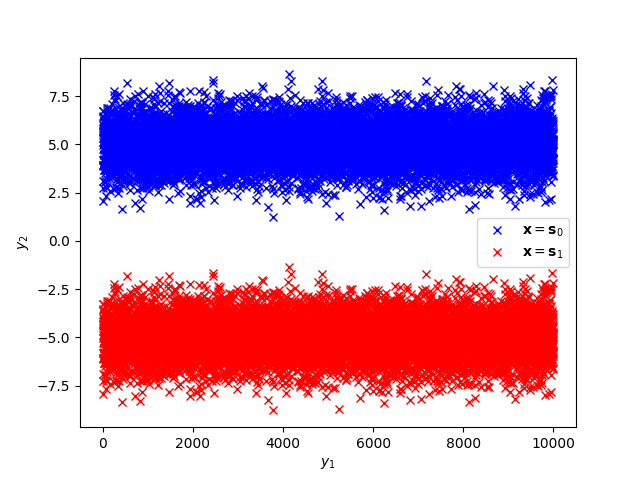
\includegraphics[width=\columnwidth]{images/scatter.png}
\caption{Scatter plot of $Y$}
\label{fig:bpsk_scatter}
\end{figure}
\item Guess how to estimate $X$ from $Y$.\\
\solution
X and Y can be estimated by decision rule\\
\begin{equation}
y \dec{1}{-1} 0
\label{eq:bpsk_decision}
\end{equation}
\item
\label{ml-ch4_sim}
Find 
\begin{equation}
	P_{e|0} = \pr{\hat{X} = -1|X=1}
\end{equation}
and 
\begin{equation}
	P_{e|1} = \pr{\hat{X} = 1|X=-1}
\end{equation}\\
\solution using decision rule in 
\begin{align}
	\pr{\hat{X} = -1|X=1} &= \pr{Y < 0|X=1}&\\
	&= \pr{AX + N < 0|X=1}&\\ 
	&= \pr{A + N < 0}&\\
	&= \pr{N < -A}\\
        &= \pr{N > A}
\end{align}
\begin{align}
	\pr{\hat{X} = 1|X=-1} &= \pr{Y > 0|X=-1}&\\
	&= \pr{N > A}
\end{align}
\begin{align*}
  \pr{N > A}&=\pr{\frac{N-0}{1}> \frac{A-0}{1}}\\&=Q(\frac{A-0}{1})=Q(A)
\end{align*}
\begin{equation}
   P_{e|0} = P_{e|1}=Q(A)\\ 
\end{equation}
\item Find $P_e$ assuming that $X$ has equiprobable symbols.\\
\solution

Since the symbols are equiprobable, it is sufficient if the error is calculated assuming that a 1 was sent.  This results in
\begin{align}
P_e &= \pr{Y < 0|X=1} = \pr{A + N < 0}
\\
&= \pr{ N< -A } = \pr{ N > A }
\label{eq:bpsk_proof_n0}
\end{align}
since $N$ has a symmetric pdf.
Let $w \sim \gauss{0}{1}$.  Then $N = \sqrt{1}w$. Substituting this in \eqref{eq:bpsk_proof_n0},
\begin{align}
P_e &=  \pr{ w > A }
\\
&= \qfunc{A}
\end{align}
%
where 
\begin{align}
\label{eq:qfunc_def}
\qfunc{x} &\define \pr{w > x}, x \ge 0 .
\\
&= \frac{1}{\pi}\int^{\frac{\pi}{2}}_{0}e^{-\frac{x^2}{2\sin^2 \theta}}\,d\theta
\end{align}


\item
Verify by plotting  the theoretical $P_e$ with respect to $A$ from 0 to 10 dB.\\
\begin{center}
\fbox{\parbox{8.2cm}{\url{https://github.com/velicharlagokulkumar/digital-communications/blob/main/codes/chapter-6/ber_snr_plot.py}}}
\end{center}
\begin{figure}[H]
\centering
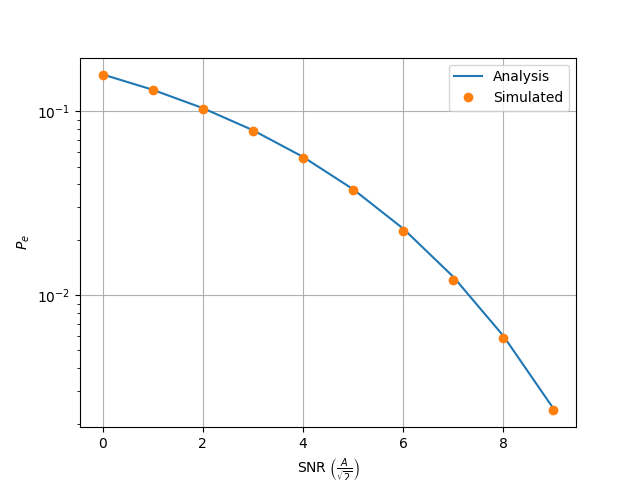
\includegraphics[width=\columnwidth]{images/ber_snr.png}
\caption{$P_e$ versus $A$ plot}
\label{fig:bpsk_pe_snr}
\end{figure}
%
\item Now, consider a threshold $\delta$  while estimating $X$ from $Y$. Find the value of $\delta$ that minimize the theoretical $P_e$.\\
\label{prob:bpsk_delta_equi}
\solution

Let $\pr{0}$, $\pr{1}$ is a probability of transmitting bit zero and bit one;\\$P_{e|0}$,$P_{e|1}$is a probability of error when detecting bit zero and bit one.


\begin{equation}
	P_e = P_{e|0} \pr{0}+P_{e|1} \pr{1}
 \label{eq:error_prob}
\end{equation}

Let $V_0$,$V_1$ be a nominal signal voltage of bit zero and  one  signal at the transmitter.
$$
\begin{aligned}
& P(e \mid 0)=\int_ \delta^{\infty} \frac{1}{\sigma \sqrt{2 \pi}} \exp \left(-\left(\nu-V_0\right)^2 / 2 \sigma^2\right) d \nu \\
& P(e \mid 1)=\int_{-\infty}^ \delta \frac{1}{\sigma \sqrt{2 \pi}} \exp \left(-\left(\nu-V_1\right)^2 / 2 \sigma^2\right) d \nu
\end{aligned}
$$
where  $\delta$ is a detection threshold.
Differentiating $P(e)$ of  \eqref{eq:error_prob} w.r.t. $T$, we arrive at
$$
\begin{gathered}
-\pr{0} \frac{1}{\sigma \sqrt{2 \pi}} \exp \left(-\left( \delta-V_0\right)^2 / 2 \sigma^2\right)+ 
\\ \pr{1} \frac{1}{\sigma \sqrt{2 \pi}} \exp \left(-\left( \delta-V_1\right)^2 / 2 \sigma^2\right)
\end{gathered}
$$
To find an optimal threshold, we equate the above expression to zero:
$$
\begin{gathered}
\pr{0} \exp \left(-\frac{\left( \delta-V_0\right)^2}{2 \sigma^2}\right)=\pr{0} \exp \left(-\frac{\left( \delta-V_1\right)^2}{2 \sigma^2}\right) \\
 \delta=\frac{V_0+V_1}{2}+\sigma^2 \ln \left(\frac{\Pr{(1)}}{\pr{0}}\right)
\end{gathered}
$$
\begin{align*}
  \implies \Pr(1) = \Pr(0) = \frac{1}{2} \\
  \implies V_0=1,V_1=-1 \\
  \therefore  \delta =0 
\end{align*}




\item Repeat the above exercise when 
\label{prob:bpsk_decision_uneqi}
	\begin{align}
		p_{X}(0) = p
	\end{align}\\
\solution 
\begin{align}
	P_e &= (1-p)P_{e|1} + pP_{e|0}
\end{align}
From Above problem we know
$$
\begin{gathered}
 \delta=\frac{V_0+V_1}{2}+\sigma^2 \ln \left(\frac{P(1)}{P(0)}\right)\\
\delta =\ln \left(\frac{1-p}{p}\right)
\end{gathered}
$$
\end{enumerate}

\section{Bivariate Random Variables: FSK}
\subsection{Two Dimensions}
     Let 
    \begin{equation}
    \mbf{y} = A\mbf{x} + \mbf{n},
    \end{equation}
    where 
    \begin{align}
    x &\in \brak{\mbf{s}_0,\mbf{s}_1}, 
    \mbf{s}_0 = 
    \begin{pmatrix}
    1 
    \\
    0
    \end{pmatrix},
    \mbf{s}_1 = 
    \begin{pmatrix}
    0 
    \\
    1
    \end{pmatrix}
    \\
    \mbf{n} &= 
    \begin{pmatrix}
    n_1
    \\
    n_2
    \end{pmatrix},
    n_1,n_2 \sim \gauss{0}{1}.
    \end{align}
    \begin{enumerate}
    \item
    Plot 
    %
    \begin{equation}
    \mbf{y}|\mbf{s}_0 \text{ and } \mbf{y}|\mbf{s}_1
    \end{equation}
    %
    on the same graph using a scatter plot.\\
    %
    \solution The following python code plots the scatter plot when $\mbf{x} = \mbf{s}_0$ and $\mbf{x} = \mbf{s}_1$ in Fig. \ref{fig:scatter_plt_y}
\begin{center}
\fbox{\parbox{8.2cm}{\url{https://github.com/velicharlagokulkumar/digital-communications/blob/main/codes/chapter-9/scatter_plot.py}}}
\end{center}
    \begin{figure}
    \centering
    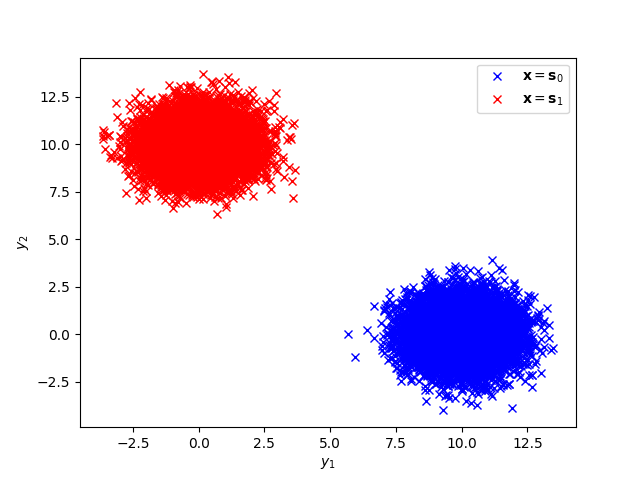
\includegraphics[width=\columnwidth]{images/scatter_plot.png}
    \caption{Scatter plot of $\vec{y}$ for $A = 10$}
    \label{fig:scatter_plt_y}
    \end{figure}
    %
    %
    \item
    For the above problem, find a decision rule for detecting the symbols $\mbf{s}_0 $ and $\mbf{s}_1$.
    \\
  \solution 
The multivariate Gaussian distribution is defined as
%
\begin{multline}
\label{eq:multivariate}
p_{\mathbf{y}}(y_1,\dots,y_k)
\\
=\frac{1}{\sqrt{\brak{2\pi}^k\abs{\bm{\sigma}}}}\exp\cbrak{-\frac{1}{2}\brak{\mathbf{y}-\bm{\mu}}^T\bm{\sigma}^{-1}\brak{\mathbf{y}-\bm{\mu}}}
\end{multline}
%
where $\bm{\mu}$ is the mean vector, $\bm{\sigma} = E\sbrak{\brak{\mathbf{x}-\bm{\mu}}\brak{\mathbf{x}-\bm{\mu}}^T}$ is the covariance matrix and $\abs{\bm{\sigma}}$ is the determinant of $\bm{\Sigma}$.
\begin{multline}
\label{eq:multivariate}
p_{\mathbf{y}}(y_1,y_2)
\\
=\frac{1}{2\pi\sqrt{\abs{\bm{\sigma}}}}\exp\cbrak{-\frac{1}{2}\brak{\mathbf{y}-\bm{\mu}}^T\bm{\sigma}^{-1}\brak{\mathbf{y}-\bm{\mu}}}
\end{multline}
\begin{multline}
p\brak{\vec{y}|s_0}
\\
=\frac{1}{2\pi\sqrt{\abs{\bm{\sigma}}}}\exp\cbrak{-\frac{1}{2}\brak{\mathbf{y}-\bm{s_0}}^T\bm{\sigma}^{-1}\brak{\mathbf{y}-\bm{s_0}}}
\label{eq:multivariate1}
\end{multline}

\begin{multline}
p\brak{\vec{y}|s_1}
\\
=\frac{1}{2\pi\sqrt{\abs{\bm{\sigma}}}}\exp\cbrak{-\frac{1}{2}\brak{\mathbf{y}-\bm{s_1}}^T\bm{\sigma}^{-1}\brak{\mathbf{y}-\bm{s_1}}}
\label{eq:multivariate2}
\end{multline}



According to the MAP criterion, assuming equiprobably symbols,optimal decison criteria can be found by equating \eqref{eq:multivariate1},\eqref{eq:multivariate2}

\begin{equation}
p\brak{\vec{y}|s_0}=p\brak{\vec{y}|s_1}
\label{eq:map_bfsk_dec1}
\end{equation}

\begin{multline*}
\frac{1}{2\pi\sqrt{\abs{\bm{\sigma}}}}\exp\cbrak{-\frac{1}{2}\brak{\mathbf{y}-\bm{s_0}}^T\bm{\sigma}^{-1}\brak{\mathbf{y}-\bm{s_0}}} \\ =\frac{1}{2\pi\sqrt{\abs{\bm{\sigma}}}}\exp\cbrak{-\frac{1}{2}\brak{\mathbf{y}-\bm{s_0}}^T\bm{\sigma}^{-1}\brak{\mathbf{y}-\bm{s_0}}}
\end{multline*}
\begin{align*}
\brak{\vec{y}-\vec{s}_0}^\top \brak{\vec{y}-\vec{s}_0} &= \brak{\vec{y}-\vec{s}_1}^\top \brak{\vec{y}-\vec{s}_1}\\
\vec{y}^\top\vec{y} - 2\vec{s}_0^\top \vec{y} + \vec{s}_0^T\vec{s}_0 &= \vec{y}^\top\vec{y} - 2\vec{s}_1^\top \vec{y} + \vec{s}_1^T\vec{s}_1\\
 2\brak{\vec{s}_1-\vec{s}_0}^\top \vec{y} &= \norm{\vec{s}_1}^2 - \norm{\vec{s}_0}^2\\
\brak{\vec{s}_1-\vec{s}_0}^\top \vec{y} &= 0\\
\myvec{-1\\1}^\top \vec{y} &= 0
\end{align*}
compare with the equation of line $ n^\top$y=c\\
\begin{align*}
  \implies y1=y2  
\end{align*}
which is decsion making line as shown in below fig
\ref{fig:bfsk_const2}

\begin{figure}[!h]
\centering
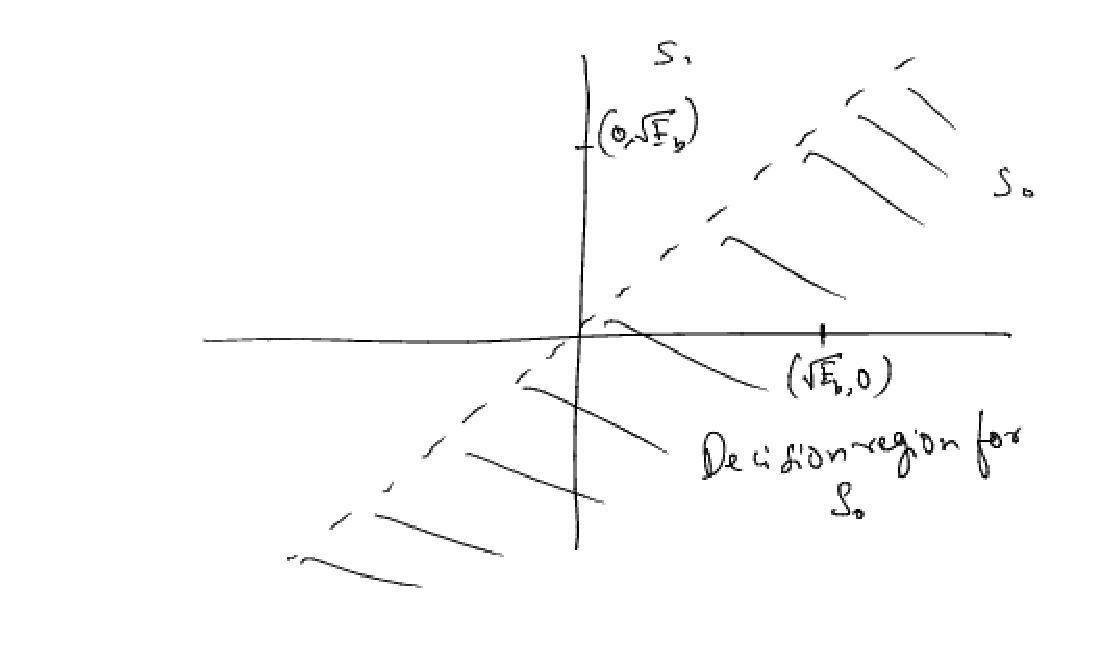
\includegraphics[width=\columnwidth]{bfsk_const.eps}
\caption{}
\label{fig:bfsk_const2}
\end{figure}
    \item
    Plot 
    \begin{equation} 
    P_e = \pr{\hat{\mbf{x}} = \mbf{s}_1|\mbf{x} = \mbf{s}_0}
    \end{equation}
    with respect to the SNR from 0 to 10 dB.
    \\
    \solution
    \begin{center}
\fbox{\parbox{8.2cm}{\url{https://github.com/velicharlagokulkumar/digital-communications/blob/main/codes/chapter-9/ber_snr_plot.py}}}
\end{center}
    \begin{figure}
        \centering
    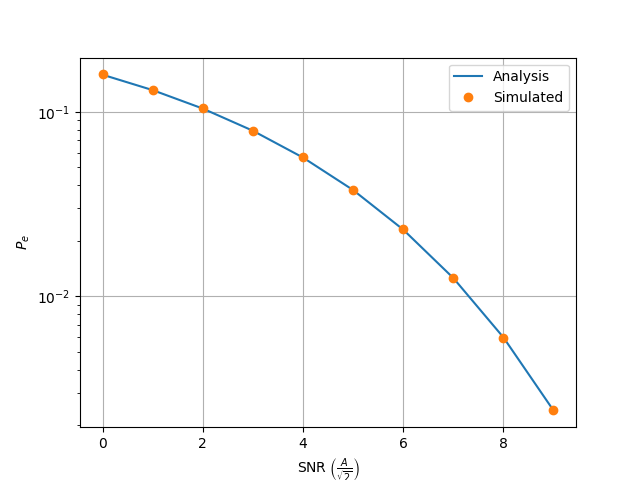
\includegraphics[width=\columnwidth]{images/ber_snr_plot.png}
        \caption{$P_e$ with respect to SNR from 0 to 10 dB}
        \label{fig:ber_snr_plot}
        \end{figure}
    %
    \item
    Obtain an expression for $P_e$. Verify this by comparing the theory and simulation plots on the same graph.
    \\
    \solution 
    \begin{align}
    P_e = \pr{\hat{\mbf{x}} = \mbf{s}_1|\mbf{x} = \mbf{s}_0}
    \end{align}
    Given that $\mbf{s}_0$ was transmitted, the received signal is
    \begin{align}
    \mbf{y}|\mbf{s}_0 = \begin{pmatrix} A \\ 0 \end{pmatrix} + \begin{pmatrix} n_1 \\ n_2 \end{pmatrix}
    \end{align}
    From decision rule, the probability of error is given by 
    \begin{align}
    P_e &= \pr{y_1 < y_2 |\mbf{s}_0} = \pr{A+n_1 < n_2}\\
    &= \pr{n_2 - n_1 > A}
    \end{align}
    Note that $n_2 - n_1 \sim \gauss{0}{2}$. Thus,
    \begin{align}
    P_e &= \pr{\sqrt{2}w > A}\\
    \pr{w > \dfrac{A}{\sqrt{2}}}\\
    \Rightarrow P_e &= \qfunc{\frac{A}{\sqrt{2}}}
    \end{align}
    where $w \sim \gauss{0}{1}$.Above code plots the $P_e$ curve in Fig. (\ref{fig:ber_snr_plot}).
    \end{enumerate}
\section{Exercises}
\subsection{BPSK}
\begin{enumerate}
\item 
The {\em signal constellation diagram} for BPSK is given by Fig. \ref{fig:bpsk_const}.  The symbols $s_0$ and $s_1$ are equiprobable.  $\sqrt{E_b}$ is the energy transmitted per bit. Assuming a zero mean additive white gaussian noise (AWGN) with variance $\frac{N_0}{2}$,
The decision rule is
\begin{equation}
y \dec{s_0}{s_1} 0
\end{equation}
Repeat the previous exercise using the MAP criterion.

%
\begin{figure}[!h]
\centering
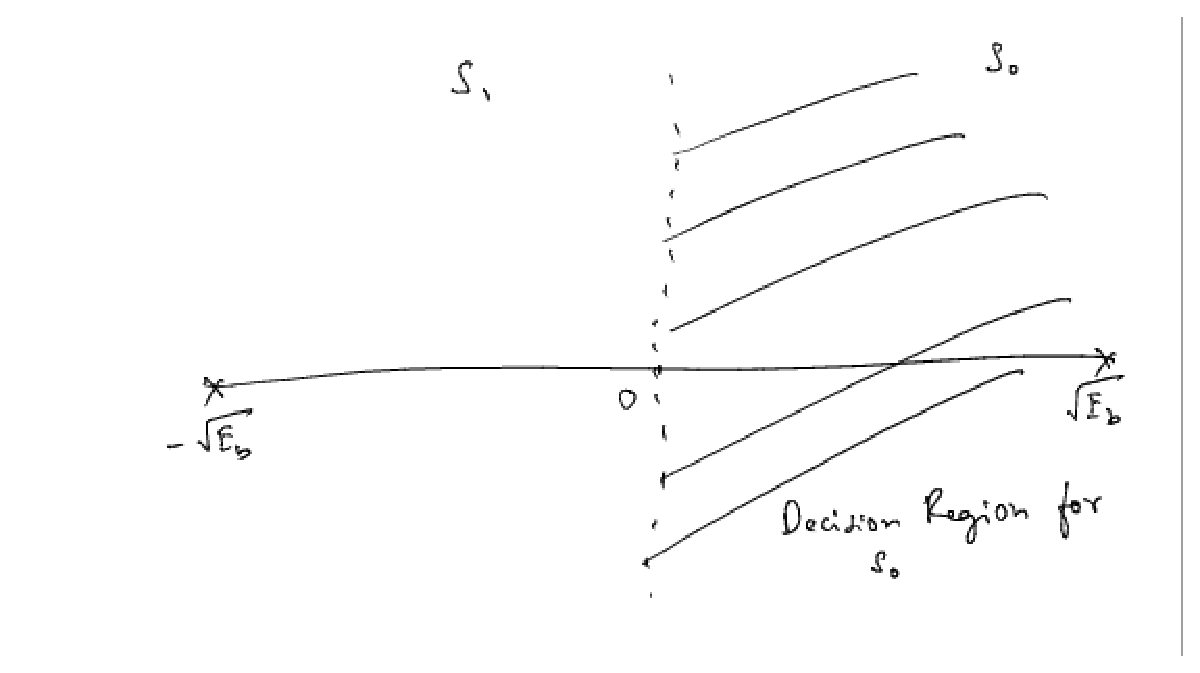
\includegraphics[width=\columnwidth]{images/bpsk.eps}
\caption{}
\label{fig:bpsk_const}
\end{figure}
\solution
According to MAP detection rule
%, we will decode the received signal  as symbol s for which  p\brak{s|y} is more.
\begin{align}
    \hat{s} &= \max_{s \in  \cbrak{s_0,s_1}} p\brak{s|y}
    \label{eq:ee18btech11042_3}
\\
    \implies p\brak{s_0|y} &\dec{s_0}{s_1} p\brak{s_1|y}
    \label{eq:ee18btech11042_4}
\end{align}
Using Bayes rule,
\begin{align}
    p\brak{s_0|y} &= \frac{p\brak{y|s_0}p\brak{s_0}}{p\brak{y}}
    \label{eq:ee18btech11042_5}
\\
    p\brak{s_1|y} &= \frac{p\brak{y|s_1}p\brak{s_1}}{p\brak{y}}
    \label{eq:ee18btech11042_6}
\end{align}
Since symbols are equi probable,  $p\brak{s_0} =  p\brak{s_1}$.  Hence the decision becomes
\begin{align}
    \frac{p\brak{y|s_0}p\brak{s_0}}{p\brak{y}} &\dec{s_0}{s_1}  \frac{p\brak{y|s_1}p\brak{s_1}}{p\brak{y}}
    \label{eq:ee18btech11042_7}
\\
    \implies p\brak{y|s_0} &\dec{s_0}{s_1} p\brak{y|s_1}
    \label{eq:ee18btech11042_8}
\end{align}
The above condition is known as the maximum-likelihood (ML) criterion.      \eqref{eq:ee18btech11042_8}
can be expressed as
{\small
\begin{align}
    \frac{1}{\sqrt{2\pi}} \exp{-\frac{(y-\sqrt{E_b})^2}{\frac{N_oN_0}{2}}}  \dec{s_0}{s_1}   
    \frac{1}{\sqrt{2\pi}} \exp{-\frac{(y+\sqrt{E_b})^2}{\frac{N_oN_0}{2}}}
    \label{eq:ee18btech11042_9}
\end{align}
}
\begin{align}
     \implies (y+\sqrt{E_b})^2 &\dec{s_0}{s_1} (y - \sqrt{E_b})^2
     \label{eq:ee18btech11042_10}
\\
    \implies y &\dec{s_0}{s_1} 0
    \label{eq:ee18btech11042_11}
\end{align}




\item The PDF of $w \sim \gauss{0}{1}$ is given by
%
\begin{equation}
p_{w}(x) = \frac{1}{\sqrt{2\pi}}\exp\brak{-\frac{x^2}{2}}, -\infty < x < \infty
\end{equation}
and the complementary error function is defined as
\begin{equation}
\operatorname {erfc} (x)={\frac {2}{\sqrt {\pi }}}\int _{x}^{\infty }e^{-t^{2}}\,dt.
\end{equation}
%
Show that 
\begin{equation}
Q(x) = \frac{1}{2}\operatorname {erfc}\left({\frac  {x}{{\sqrt  {2}}}}\right)
\end{equation}
\solution 
we know that
\begin{equation}
\operatorname {erfc} (x)={\frac {2}{\sqrt {\pi }}}\int _{x}^{\infty }e^{-t^{2}}\,dt.
\end{equation}
\begin{equation}
Q(u) = \frac{1}{2\pi}\int^{\infty}_{u}e^{-\frac{t^2}{2}}\,dt
\end{equation}

\begin{align}
 u=\frac{u'}{\sqrt{2}}  ,u'=\sqrt{2}u\\
 du=\frac{du'}{\sqrt{2}}
\end{align}

\begin{align}
\operatorname {erfc} (x)&={\frac {2}{\sqrt {\pi }}}\int _{x}^{\infty }e^{-u^{2}/2}\,\frac{du'}{\sqrt{2}}  \\
&={\frac {2}{\sqrt {2\pi }}}\int _{\sqrt{2}x}^{\infty }e^{-u^{2}/2}\,du'\\
\operatorname {erfc} (x)&=2Q(\sqrt{2}x)\\
\implies Q(\sqrt{2}x)&=\frac{1}{2}\operatorname {erfc} (x)
\end{align}


\begin{equation}
\therefore Q(x) = \frac{1}{2}\operatorname {erfc}\left({\frac  {x}{{\sqrt  {2}}}}\right)
\end{equation}


\item
Verify the bit error rate (BER) plots for BPSK through simulation and analysis for 0 to 10 dB. \\
\solution
The following code yields Fig. \ref{fig:bpsk_ber}
\begin{center}
\fbox{\parbox{8.2cm}{\url{https://github.com/velicharlagokulkumar/digital-communications/blob/main/codes/chapter-10/bpsk_ber.py}}}
\end{center}
%	\
\begin{figure}[!h]
\centering
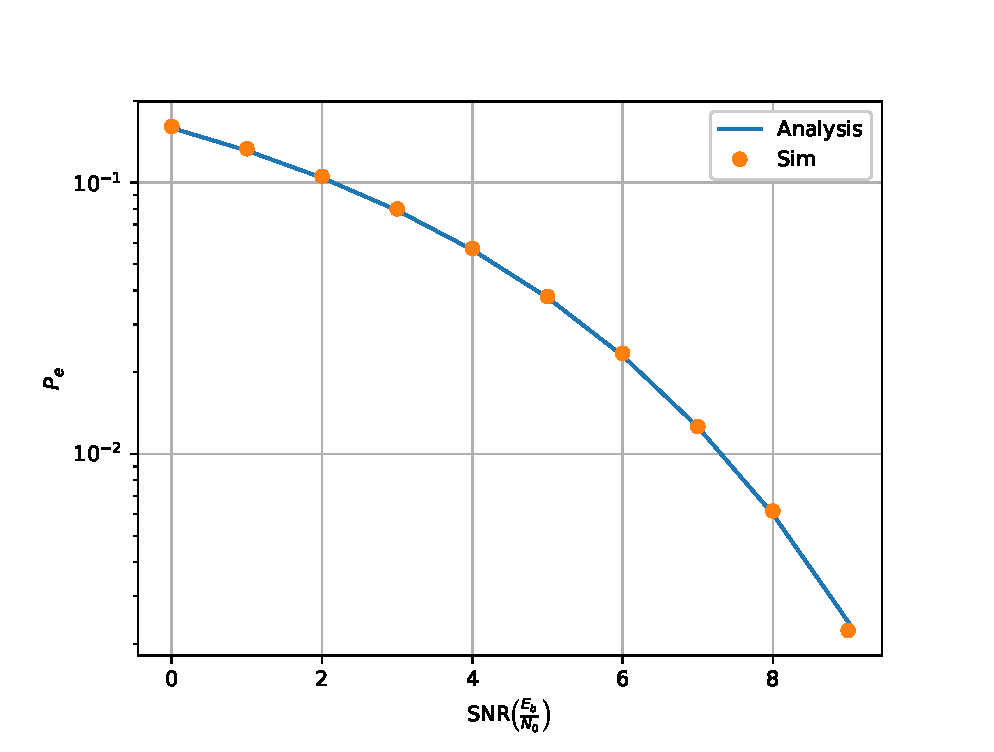
\includegraphics[width=\columnwidth]{images/bpsk2.eps}
\caption{}
\label{fig:bpsk_ber}
\end{figure}
\item
Show that
\begin{equation}
Q(x) = \frac{1}{\pi}\int^{\frac{\pi}{2}}_{0}e^{-\frac{x^2}{2\sin^2 \theta}}\,d\theta
\end{equation}
\solution 
\solution Consider the bivariate gaussian distribution of $X,Y \sim \gauss{0}{1}$,
\begin{equation}
	p_{X,Y}(x,y) = \frac{1}{2\pi}\exp\left(-\frac{x^2+y^2}{2}\right)
	\label{eq:bivariate_std_gaussian_pdf}
\end{equation}
Q-function can be expressed with \eqref{eq:bivariate_std_gaussian_pdf} as
\begin{align}
	Q(z) &= \int_{z}^{\infty}\int_{-\infty}^{\infty} p_{X,Y}(x,y) \,dx\,dy \\
	\label{eq:qfunc_biv_integ}
	&= \frac{1}{2\pi}\int_{z}^{\infty}\int_{-\infty}^{\infty} \exp\left(-\frac{x^2+y^2}{2}\right) \,dx\,dy
\end{align}
Transforming the integral in \eqref{eq:qfunc_biv_integ} to polar coordinates $(r,\theta)$ for $z > 0$,
\begin{align}
	Q(z) &= \frac{1}{2\pi}\int_{-\frac{\pi}{2}}^{\frac{\pi}{2}}\int_{\frac{z}{\sin\theta}}^{\infty} \exp\left(-\frac{r^2}{2}\right)r \,dr\,d\theta\\
	&= \frac{1}{2\pi}\int_{-\frac{\pi}{2}}^{\frac{\pi}{2}} \exp\left(-\frac{z^2}{2\sin^2\theta}\right) \,d\theta\\
	&= \frac{1}{\pi}\int_{0}^{\frac{\pi}{2}} \exp\left(-\frac{z^2}{2\sin^2\theta}\right) \,d\theta \text{ , for $z > 0$}
\end{align}
\end{enumerate}



\subsection{Coherent BFSK}
\begin{enumerate}
\item
The signal constellation for binary frequency shift keying (BFSK) is given in Fig. \ref{fig:bfsk_const}.The received symbols are given by 
\begin{align}
\mathbf{y}|s_0 = 
\myvec{
\sqrt{E_b} \\
0
}
+
\myvec{
 n_{1}\\
n_{2}
},
\end{align}
and 
\begin{align}
\mathbf{y}|s_1 = 
\myvec{
0\\
\sqrt{E_b} 
}
+
\myvec{
n_{1}\\
 n_{2}
},
\end{align}
where $n_1,n_2 \sim \gauss{0}{\frac{N_0}{2}}$. and
$
\mathbf{y} = 
\myvec{
y_{1}\\
 y_{2}
}
$.

\begin{figure}[!h]
\centering
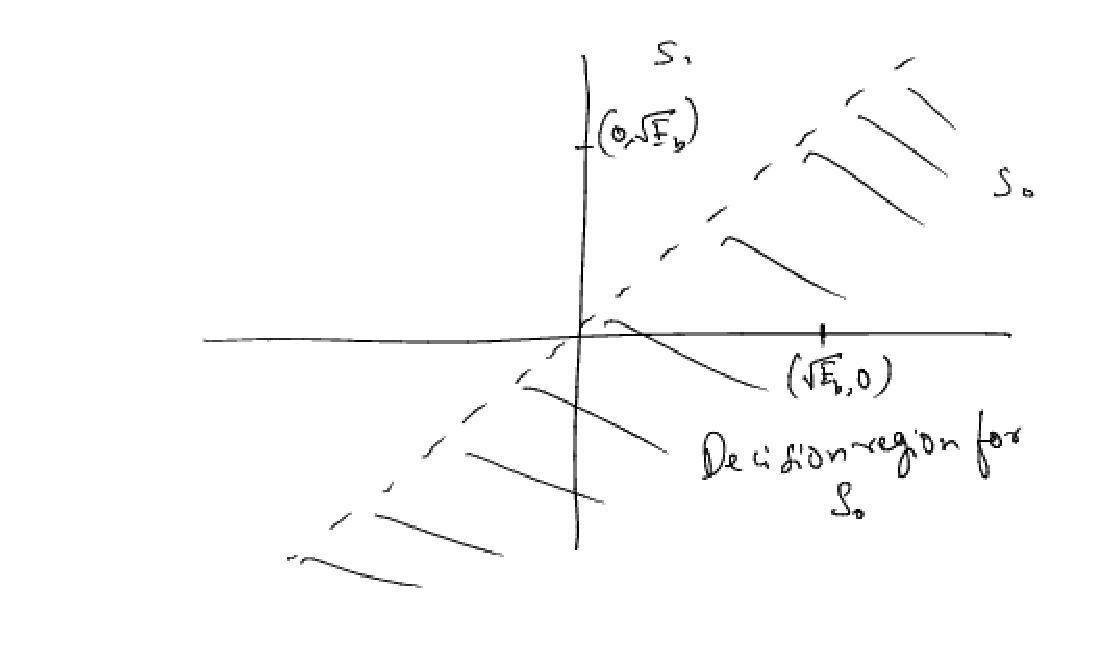
\includegraphics[width=\columnwidth]{bfsk_const.eps}
\caption{}
\label{fig:bfsk_const}
\end{figure}
decision rule for BFSK from Fig. \ref{fig:bfsk_const}. is
\begin{equation}
y_1 \dec{s_0}{s_1} y_2
\end{equation}
Repeat the above using the MAP criterion.\\
\solution 
 The multivariate Gaussian distribution is defined as
%
\begin{multline}
\label{eq:multivariate}
p_{\mathbf{x}}(x_1,\dots,x_k)
\\
=\frac{1}{\sqrt{\brak{2\pi}^k\abs{\bm{\sigma}}}}\exp\cbrak{-\frac{1}{2}\brak{\mathbf{x}-\bm{\mu}}^T\bm{\sigma}^{-1}\brak{\mathbf{x}-\bm{\mu}}}
\end{multline}
%
where $\bm{\mu}$ is the mean vector, $\bm{\sigma} = E\sbrak{\brak{\mathbf{x}-\bm{\mu}}\brak{\mathbf{x}-\bm{\mu}}^T}$ is the covariance matrix and $\abs{\bm{\sigma}}$ is the determinant of $\bm{\Sigma}$.
The PDF of the {\em bivariate} Gaussian is
{\small
\begin{multline}
\label{eq:bivariate}
p(x,y)= \frac{1}{2\pi \sigma_x\sigma_y\sqrt{1-\rho^2}}\exp\lsbrak{-\frac{1}{2\brak{1-\rho^2}}}
\\
\times \rsbrak{\cbrak{\frac{\brak{x-\mu_x}^2}{\sigma_x^2}+\frac{\brak{y-\mu_y}^2}{\sigma_y^2}-\frac{2\rho\brak{x-\mu_x}\brak{y-\mu_y}}{\sigma_x\sigma_y}}}
\end{multline}
}
%
where
%
\begin{align}
%\bm{\mu}=
\bm{\mu}=
\begin{pmatrix}
\mu_x \\
\mu_y
\end{pmatrix},
\bm{\Sigma} = 
\begin{pmatrix}%[r]
\sigma_x^2 & \rho\sigma_x\sigma_y \\
\rho\sigma_x\sigma_y & \sigma_y^2
\end{pmatrix}
\end{align}

According to the MAP criterion, assuming equiprobably symbols,
%
\begin{equation}
\label{eq:map_bfsk_dec}
%p\brak{\mathbf{y}|s_0} \dec{s_0}{s_1} p\brak{\mathbf{y}|s_1}
p\brak{s_0|\vec{y}} \dec{s_0}{s_1} p\brak{s_1|\vec{y}}
\end{equation}
Use \eqref{eq:bivariate} in \eqref{eq:map_bfsk_dec}  to obtain \eqref{eq:map_bfsk_dec}.
\\

\begin{definition}
The joint PDF of $X,Y$ is given by
\begin{multline}
\label{eq:bivariate2}
p(x,y)= \frac{1}{2\pi \sigma_x\sigma_y\sqrt{1-\rho^2}}\exp\lsbrak{-\frac{1}{2\brak{1-\rho^2}}}
\\
\times \rsbrak{\cbrak{\frac{\brak{x-\mu_x}^2}{\sigma_x^2}+\frac{\brak{y-\mu_y}^2}{\sigma_y^2}-\frac{2\rho\brak{x-\mu_x}\brak{y-\mu_y}}{\sigma_x\sigma_y}}}
\end{multline}
%
where
\begin{align}
\mu_x &= E\sbrak{X},
\sigma_x^2 = \text{var}\brak{X},
\rho = \frac{E\sbrak{\brak{X - \mu_x}\brak{Y-\mu_y}}}{\sigma_x\sigma_y}.
\end{align}
\end{definition}
%






\item
Derive and plot the probability of error.  Verify through simulation.

\solution Given that $s_0$ was transmitted, the received symbols are
\begin{align}
\mathbf{y}|s_0 = 
\begin{pmatrix}
\sqrt{E_b} \\
0
\end{pmatrix}
+
\begin{pmatrix}
 n_{1}\\
n_{2}
\end{pmatrix},
\end{align}
From \eqref{eq:map_bfsk_dec}, 
the probability of error is given by
\begin{align}
P_e &= \pr{y_1 < y_2|s_0} = \pr{\sqrt{E_b} + n_1 < n_2}
\\
&= \pr{ n_2-n_1 > \sqrt{E_b} } 
\label{eq:bfsk_proof_n0}
\end{align}
Note that $n_2-n_1 \sim \gauss{0}{N_0}$. Thus, 
\begin{align}
P_e &= \pr{ \sqrt{N_0}w > \sqrt{E_b} }  =  \pr{ w > \sqrt{\frac{E_b}{N_0}} }
%= \pr{ X > \sqrt{E_b} }
\\
\implies 
P_e & = \qfunc{\sqrt{\frac{E_b}{N_0}}}
\end{align}
where 
%$X \sim \gauss{0}{N_0}$
%\\
$w \sim \gauss{0}{1}$.  
%Then $X = \sqrt{N_0}w$. Substituting this in \eqref{eq:fsk_proof_n0},
%where $\qfunc{x} \define \pr{w > x}, x \ge 0$.
%
The following code plots the BER curves in Fig. \ref{fig:bfsk_ber}
\begin{center}
\fbox{\parbox{8.2cm}{\url{https://github.com/velicharlagokulkumar/digital-communications/blob/main/codes/chapter-10/bfsk_ber.py}}}
\end{center}


\begin{figure}[!h]
\centering
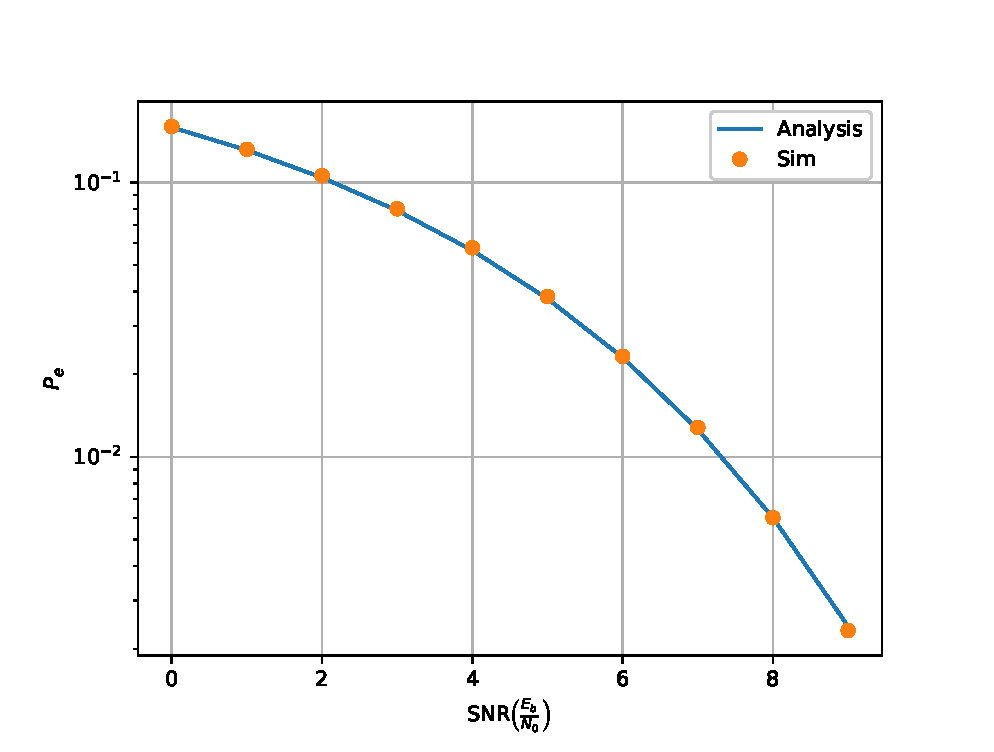
\includegraphics[width=\columnwidth]{bfsk_ber.eps}
\caption{}
\label{fig:bfsk_ber}
\end{figure}


\end{enumerate}
\end{document}














